\documentclass[12pt,a4, oneside, brazil]{article}
\usepackage{graphicx} 
\usepackage[portuguese]{babel}
\usepackage[utf8]{inputenc}
\usepackage[lmargin=3cm,tmargin=3cm,rmargin=2cm,bmargin=2cm]{geometry} 
\usepackage{hyperref}
\usepackage{float}


\title{Impressoras e Scanners}
\author{Diogo Siqueira Santos, Enzo Picanço Alberoni, Mariana Cossetti Dalfior, Mateus do Nascimento Viana}
\date{5 de Maio 2023}

\begin{document}
	\thispagestyle{empty}
	
	\begin{center}
	
		\Large \textbf{Universidade Estadual do Norte Fluminense Darcy Ribeiro (UENF)}
		\vspace{3cm}
		
		\Large \textbf{Diogo Siqueira Santos, Enzo Picanço Alberoni, Mariana Cossetti Dalfior, Mateus do Nascimento Viana}
		\vspace{7cm}
		
		\Large \textbf{\textbf{Impressoras e Scanners}}
	\end{center}

	\begin{center}
		\vspace{7cm}
		\textbf{Campos dos Goytacazes, Rio de Janeiro \\ 2023}
	\end{center}

\newpage

	\nocite{Tanenbaum2013}
	\nocite{Suprivix2022}
	\nocite{Silva2015}
	\nocite{Copygreen2022}
	 
	\section{Introdução}
	As impressoras e os scanners são dispositivos de E/S (entrada /saída) ou I/O (input/output) muito importantes na área de tecnologia, visto que, são dispositivos fundamentais para a realização de atividades essenciais. Com o avanço da tecnologia, as impressoras e scanners estão cada vez mais integrados aos computadores, permitindo que documentos sejam impressos e digitalizados com grande rapidez e facilidade. Neste sentido, é importante compreender como esses dispositivos funcionam e quais são suas principais características.	
	
	\section{Impressoras}
		\subsection{História}
		A impressora é um equipamento indispensável nos dias atuais, mas sua invenção e desenvolvimento foram frutos de pesquisas e avanços tecnológicos. Chester Floyd Carlson, um físico dos Estados Unidos, é considerado o inventor das impressoras, percebeu a necessidade de um equipamento capaz de reproduzir textos e imagens através de cópias em fotos e, para isso, utilizou a tecnologia da eletrografia. 
		
		Carlson introduziu a eletricidade estática em cilindros sensíveis às fotografias, que registravam o material a ser impresso através da imagem do documento original refletida por um sistema de espelhos. Esse cilindro arquivava o desenho da imagem original e um toner era ativado através da carga elétrica presente na imagem. Em um sistema de força, temperatura e eletricidade, o toner era levado ao papel, depositando o desenho da fotocópia feita do material original. Esse sistema de impressão, conhecido como Xerox, foi pioneiro no foco científico e comercial para equipamentos de reprodução de material gráfico. Com o avanço tecnológico, outras impressoras mais rápidas foram desenvolvidas a partir de 1953.
		
		\subsection{Impressoras matricial}
		A impressora matricial é uma tecnologia de impressão pioneira, que ainda é encontrada em uso em muitos estabelecimentos. Embora tenha sido amplamente superada por tecnologias de impressão mais avançadas, ela ainda possui uma base de usuários fiéis devido à sua durabilidade e baixo custo de manutenção e suprimentos.
		
		\begin{figure}[H]
			\centering
			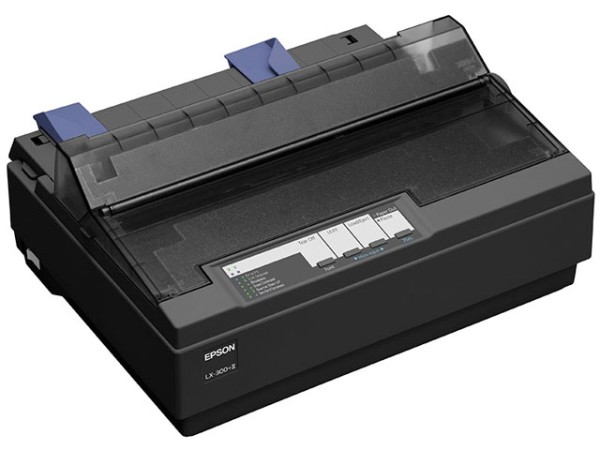
\includegraphics[width=8cm]{matricial}
			\caption{Impressora matricial}
			\label{fig:monomodo}
		\end{figure}
	
		As impressoras matriciais, que se enquadram na categoria de impressoras de impacto, utilizam predominantemente duas tecnologias distintas como base para seu funcionamento:
			\subsubsection{Impressora margarida}
			O funcionamento das impressoras margarida é semelhante ao das máquinas de escrever clássicas e atualmente é considerado pouco comum no mercado. A cabeça de impressão contém caracteres em relevo e se move de acordo com o caractere a ser impresso. Por exemplo, se a letra "A" for solicitada, a cabeça posicionará essa letra sobre o papel. Para imprimir, o caractere pressiona uma fita com tinta contra o papel, em um movimento rápido e semelhante a uma batida de martelo.
			
			\begin{figure}[H]
				\centering
				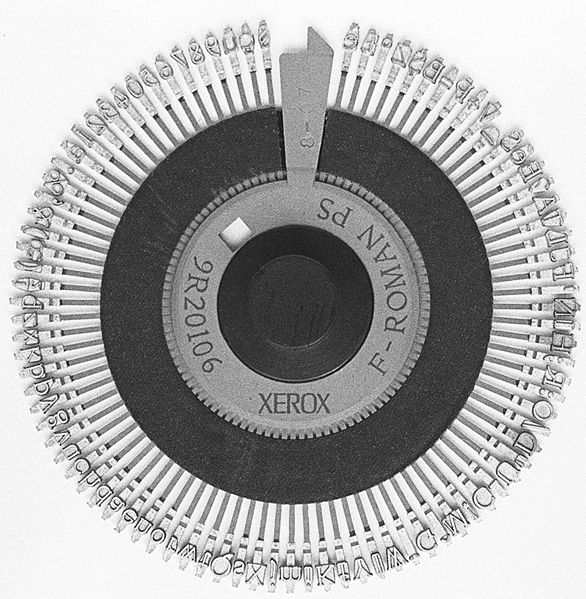
\includegraphics[width=8cm]{margarida}
				\caption{Impressora margarida}
				\label{fig:monomodo}
			\end{figure}
			
			\subsubsection{Impressora de agulha}
			
			A impressora de agulha é mais comum e por isso é conhecido simplesmente como "impressora matricial" ou "impressora de matriz de pontos". Nessa tecnologia, a cabeça de impressão contém pequenas agulhas que são controladas eletronicamente e pressionam a fita de tinta contra o papel para formar a impressão. Diferente da tecnologia anterior, os caracteres são formados por pequenos pontos, permitindo também a impressão de imagens e gráficos, embora com algumas limitações.
			
			\begin{figure}[H]
				\centering
				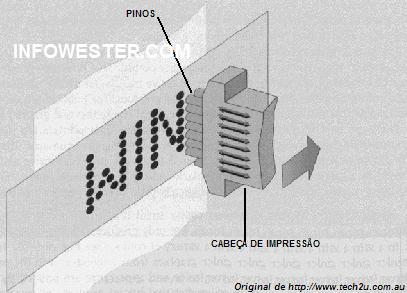
\includegraphics[width=8cm]{agulha}
				\caption{Funcionamento da impressora de agulha}
				\label{fig:monomodo}
			\end{figure}
		
		\subsection{Impressoras a laser}
		A impressora a laser é uma inovação bastante significativa na história da impressão, sendo altamente flexível, de excelente qualidade, com alta velocidade e custo moderado, tudo isso em um único dispositivo compacto. A tecnologia utilizada na impressora a laser é muito semelhante às máquinas de fotocópia, tanto que muitas empresas fabricam dispositivos que combinam impressão, cópia e, às vezes, fax.
		
		O coração da impressora a laser é um tambor rotativo ou correia, dependendo do modelo. Esse tambor é revestido com um material fotossensível e recebe uma carga elétrica de até cerca de 1.000 volts no início de cada ciclo de página. Um laser passa pelo comprimento do tambor e é refletido por um espelho octogonal rotativo. O laser é modulado para produzir um padrão de pontos escuros e claros que atinge apenas os pontos que perdem sua carga elétrica.
		
				\begin{figure}[H]
					\centering
					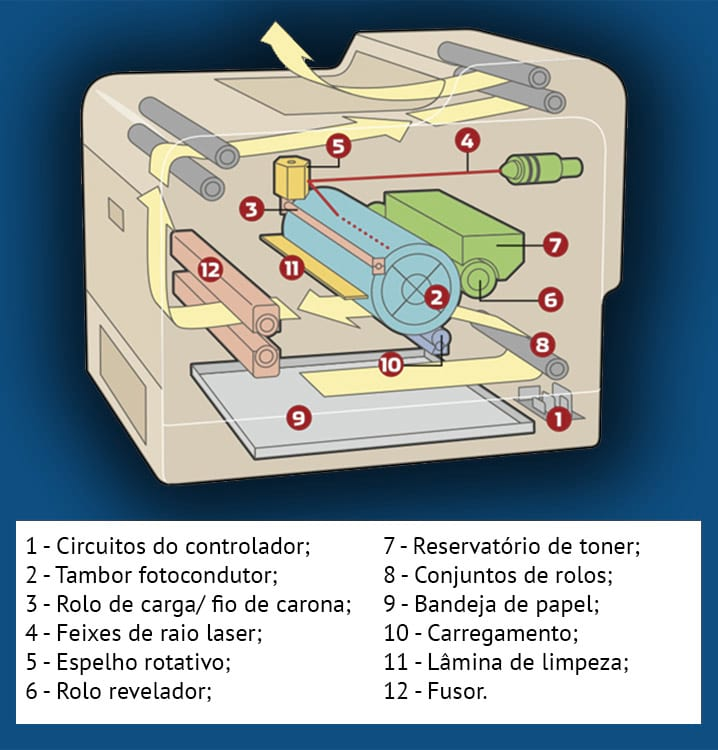
\includegraphics[width=13cm]{laser}
					\caption{Interno da impressora a laser}
					\label{fig:monomodo}
				\end{figure}
		
		A impressora a laser é uma complexa combinação de física, química, engenharia mecânica e engenharia ótica. A tecnologia envolve um tambor que gira para permitir a impressão de uma linha de pontos carregados, atraindo o toner preto para formar uma imagem naqueles pontos. Em seguida, o papel é pressionado contra o tambor revestido de toner e passa por rolamentos aquecidos para fixar a imagem permanentemente. Após a impressão, o tambor é descarregado e raspado para remover qualquer resíduo de toner, preparando-o para imprimir a próxima página. Há vários fabricantes de mecanismos de impressão no mercado, que são combinados com eletrônica e software personalizados para criar impressoras a laser completas. A eletrônica inclui uma CPU rápida e megabytes de memória para conter um mapa de bits de uma página inteira e fontes especiais. As impressoras a laser de alta resolução podem imprimir fotografias em preto e branco, mas o processo é mais complicado do que se imagina, pois a imagem digitalizada em 600 dpi contém valores de cinza que não podem ser impressos diretamente na resolução de 600 dpi da impressora.
		
		Para imprimir imagens que contêm valores de cinza, é comum utilizar a técnica do meio-tom, que também é empregada na produção de cartazes comerciais. Essa técnica divide a imagem em células de meios-tons, geralmente de tamanho 6 x 6 pixels. Cada célula pode conter entre 0 e 36 pixels pretos, e a percepção visual do olho humano faz com que células com mais pixels pretos pareçam mais escuras do que células com menos pixels pretos. Para representar valores de cinza na faixa de 0 a 255, essa faixa é dividida em 37 zonas. Valores de cinza de 0 a 6 são representados na zona 0, valores de 7 a 13 na zona 1, e assim por diante, sendo a zona 36 um pouco menor do que as outras devido a 256 não ser um número divisível exatamente por 37. Quando um valor de cinza é encontrado na zona 0, a célula de meio-tom correspondente é deixada em branco no papel. Valores de outras zonas são impressos com uma quantidade de pixels pretos que corresponde à sua zona, conforme ilustrado em diferentes figuras. É importante destacar que a utilização da técnica de meio-tom em uma imagem digitalizada em 600 dpi reduz sua resolução efetiva a 100 células por polegada, conhecida como frequência de tela de meio-tom, medida em lpi (linhas por polegada).
		
				\begin{figure}[H]
					\centering
					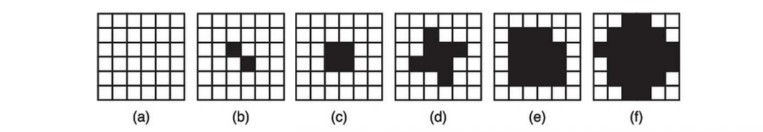
\includegraphics[width=15cm]{cinza}
					\caption{Pontos de meio-tom poro várias faixas de escala de cinza}
					\label{fig:cinza}
				\end{figure}
		
			\subsubsection{Impressão colorida}
			É cada vez mais comum encontrar impressoras a laser coloridas, embora a maioria seja monocromática. No entanto, é importante entender que a impressão colorida não é um processo trivial e pode ser visto de duas maneiras: por luz transmitida ou por luz refletida. As imagens por luz transmitida, como as exibidas em monitores, são compostas pela superposição linear das três cores primárias aditivas: vermelho, verde e azul. Por outro lado, as imagens por luz refletida, como as fotografias em cores e as fotos em revistas, são compostas pela superposição linear das três cores subtrativas primárias: ciano, magenta e amarelo.
			
			Embora teoricamente todas as cores possam ser produzidas misturando as tintas ciano, magenta e amarela, na prática, é difícil obter essas tintas com a pureza necessária para absorver toda a luz e produzir um preto verdadeiro. Portanto, a maioria dos sistemas de impressão em cores utiliza quatro tintas: ciano, magenta, amarela e preta, e são conhecidos como impressoras CMYK. O conjunto completo de cores que uma impressora ou um monitor pode produzir é chamado de gama.
			
			No entanto, nenhum dispositivo tem uma gama que se iguale à do mundo real, pois cada cor vem em apenas 256 intensidades no máximo, o que equivale a apenas 16.777.216 cores discretas. Imperfeições na tecnologia também reduzem ainda mais esse total e as cores restantes nem sempre estão uniformemente espaçadas no espectro de cores. Além disso, a percepção da cor está relacionada ao modo de funcionamento dos bastões e cones na retina, e não apenas com a física da luz.
			
			Isso torna a conversão de uma imagem colorida que parece boa na tela em uma imagem impressa idêntica um processo desafiador, pois existem várias diferenças entre monitores e impressoras. Alguns desses problemas incluem a diferença entre a luz transmitida e a luz refletida, a necessidade de utilizar meios-tons nas impressoras, a diferença entre o fundo preto do monitor e o fundo claro do papel, e a diferença entre as gamas RGB do monitor e as gamas CMYK da impressora.
			
		\subsection{Impressora a jato de tinta}
		As impressoras a jato de tinta são uma escolha popular para impressão em casa devido ao seu baixo custo. Elas possuem uma cabeça de impressão móvel que é varrida horizontalmente pelo papel através de uma correia enquanto minúsculas gotículas de tinta são espirradas por esguichos. Com um volume de cerca de 1 picolitro, são necessárias cerca de 100 milhões dessas gotículas para formar uma única gota d'água.
		
		Existem dois tipos principais de impressoras a jato de tinta: piezelétricas e térmicas. As impressoras piezelétricas usam um cristal especial perto da câmara de tinta que se deforma ligeiramente quando uma tensão elétrica é aplicada, forçando uma gotícula de tinta a sair pelo esguicho. A tensão controla o tamanho da gotícula. As impressoras térmicas, por outro lado, contêm um minúsculo resistor dentro de cada esguicho que se aquece rapidamente quando uma tensão elétrica é aplicada. Isso faz com que a tinta entre em ebulição e forme uma bolha de gás que empurra a tinta para o papel. A velocidade da impressora é limitada pela velocidade com que o ciclo de aquecimento/resfriamento pode ser repetido.
		
		As impressoras a jato de tinta geralmente têm resoluções de pelo menos 1.200 dpi e, no máximo, 4.800 dpi. Elas são baratas e silenciosas, mas também são lentas e requerem cartuchos de tinta caros. No entanto, quando usadas para imprimir fotografias em alta resolução em papel fotográfico de alta qualidade, podem produzir resultados semelhantes aos das fotografias convencionais.
		
		Para obter os melhores resultados, é necessário usar tinta e papel especiais. As tintas à base de corantes produzem cores brilhantes, mas tendem a desbotar quando expostas à luz UV. As tintas à base de pigmentos não desbotam com o tempo, mas não são tão brilhantes e podem entupir os bicos injetores. Para imprimir fotografias, é recomendado o uso de papel lustroso ou revestido para conter as gotículas de tinta e evitar que se espalhem.
		
		\subsection{Impressoras especiais}
		Embora as impressoras a jato de tinta e a laser sejam amplamente utilizadas para impressão em ambientes domésticos e empresariais, existem outros tipos de impressoras que são usados em diferentes cenários, com requisitos específicos de qualidade de cor, preço e outras características.
		
			\subsubsection{Impressora de tinta sólida}
			
			Esse tipo de impressoras utilizam tinta sólida em vez de tinta líquida para imprimir textos e imagens em papel. A tinta sólida é aquecida dentro de um cartucho e transferida para o papel por meio de um rolo aquecido, que derrete a tinta e a deposita na superfície do papel.
			
			Em comparação com os modelos convencionais, as impressoras de tinta sólida possuem algumas vantagens. Em primeiro lugar, elas são mais resistentes e duráveis, já que a tinta sólida não se espalha ou vaza como a tinta líquida. Além disso, a impressão em tinta sólida oferece uma qualidade de cor mais nítida e precisa, com menos borrões e manchas.
			 
			As impressoras de tinta sólida também são mais amigáveis ao meio ambiente, pois consomem menos energia e geram menos resíduos. No entanto, elas apresentam algumas desvantagens, como um custo inicial mais alto e uma variedade limitada de modelos e marcas disponíveis no mercado. Além disso, a tinta sólida pode levar mais tempo para aquecer e começar a imprimir do que as tintas líquidas.
			
			\subsubsection{Impressora a cera}
			
			As impressoras de cera são uma categoria de impressoras que utilizam uma tecnologia similar às de tinta sólida. Elas empregam tinta sólida à base de cera, que é aquecida em um cartucho e transferida para o papel através de um cabeçote de impressão.
			
		 	As impressoras a cera são capazes de imprimir em uma grande variedade de mídias, como papel sintético, papel revestido e poliéster, e oferecem alta resistência a água, abrasão e desbotamento. Adicionalmente, as impressoras de cera possuem velocidade de impressão superior a muitas outras tecnologias, como as impressoras jato de tinta, utilizando uma tecnologia de impressão por transferência térmica e uma tinta sólida à base de cera.
			
			Entretanto, as impressoras de cera possuem algumas desvantagens, tais como o custo de produção elevado em relação a outras tecnologias de impressão e a incapacidade de imprimir em cores, o que limita sua utilização em certas aplicações.
			
			\subsubsection{Impressora por sublimação de corante ou tinta}
			Uma impressora sublimática é um equipamento de impressão que utiliza o processo de sublimação para transferir imagens de alta qualidade para materiais como tecidos, papéis, canecas e outros produtos. Esse tipo de impressora é amplamente utilizado na indústria têxtil, publicidade, decoração de interiores, entre outras áreas.
			
			O funcionamento da impressora sublimática é relativamente simples. Ela utiliza tintas especiais que são transformadas em vapor quando aquecidas. Esse vapor é então transferido para a superfície do material, onde se solidifica, formando uma imagem nítida e durável. Para garantir a precisão e a qualidade da imagem, a impressora sublimática utiliza um sistema de cabeças de impressão de alta resolução, que podem imprimir milhões de pontos por segundo.
			
			Os componentes da impressora sublimática incluem um sistema de alimentação de tinta, um sistema de cabeças de impressão, um mecanismo de transporte de papel ou tecido e um sistema de aquecimento. A alimentação de tinta é feita por meio de cartuchos ou reservatórios, que são conectados às cabeças de impressão por tubos de tinta. 
			
			Um dos principais benefícios da impressora sublimática é a qualidade de imagem que ela proporciona. Como as tintas são transferidas para o material em forma de vapor, elas conseguem penetrar nas fibras do tecido ou do papel, criando uma imagem vibrante e de alta definição. Além disso, a sublimação é um processo permanente, o que significa que a imagem não desbota ou se desgasta com o tempo.
			
			Portanto, a impressora sublimática é uma ferramenta essencial para empresas que desejam criar produtos personalizados e de alta qualidade. Tendo em vista que ela possui a capacidade de imprimir em uma ampla variedade de materiais, a sua qualidade de imagem superior e também a sua durabilidade devido ao processo de sublimação
			
			\subsubsection{Impressora térmica}
			
			Uma impressora térmica é um dispositivo de última geração que usa o calor como meio para imprimir imagens ou texto em um papel térmico especial, que é reativo ao calor e não requer tinta ou toner. Através de uma reação química completamente silenciosa causada pelo calor produzido pelos resistores localizados no cabeçote da impressora, o papel especial libera cor e cria a imagem. O termo "impressora térmica" surgiu na década de 1940, quando o engenheiro eletricista e físico americano Jack St. Clair Kilby criou o primeiro modelo desta categoria, e agora existem inúmeras marcas e modelos disponíveis no mercado.
			
			Uma impressora térmica direta utiliza uma cabeça de impressão composta por vários pinos pequenos que aplicam calor seletivamente ao papel sensível ao calor. Essa aplicação de calor ativa produtos químicos sensíveis ao calor no papel ou queima o papel para criar um design.
			Normalmente, as impressoras térmicas diretas são utilizadas para produzir impressões em uma única cor, preto, embora algumas também ofereçam a opção de uma segunda cor.
			
			Por sua vez, as impressoras de transferência térmica aplicam calor a uma fita encerada que é colocada entre o cabeçote de impressão e o material a ser impresso. O calor derrete a cera, que é transferida e resfriada imediatamente no material impresso, produzindo um resultado sem manchas.
			As impressoras de transferência térmica são frequentemente usadas para marcar etiquetas plásticas com códigos de barras. Esse método de impressão produz um produto final mais durável, com menor probabilidade de manchas ou desbotamento, além de ser capaz de imprimir em velocidades muito altas.
			
			A impressora térmica é amplamente utilizada em vários setores, incluindo lojas, comércios, indústrias e empresas de entretenimento, para imprimir documentos como cupons fiscais, bilhetes de passagem e etiquetas de identificação. Algumas das vantagens dessas impressoras incluem velocidade de impressão mais rápida, custos de impressão reduzidos, manuseio simples, baixo custo de manutenção, maior robustez, tamanho compacto e conectividade.

	\section{Scanners}

	Um scanner é um dispositivo eletrônico que permite digitalizar documentos, imagens e outros tipos de mídia física, transformando-os em formato digital para serem armazenados, processados e compartilhados no computador. O processo de digitalização envolve a conversão de uma imagem ou documento físico em um formato de imagem digital que pode ser salvo, editado e compartilhado eletronicamente.
	
	Existem diversos tipos de scanners, desde os modelos de mesa aos scanners portáteis que podem ser facilmente transportados para qualquer lugar. Os scanners modernos possuem recursos adicionais, como alimentadores automáticos de documentos, que permitem digitalizar várias páginas de um documento de uma só vez, além de permitir a digitalização de negativos de filmes e slides.
	
	Para digitalizar uma imagem ou documento, o scanner utiliza uma fonte de luz, geralmente um LED ou lâmpada, para iluminar a superfície do documento. A luz reflete da superfície do documento e é capturada por um conjunto de sensores, geralmente CCD (Charge-Coupled Device) ou CIS (Contact Image Sensor), que transformam a luz em sinais elétricos.
	
	Os sinais elétricos são então processados por um processador interno no scanner e convertidos em um formato de imagem digital, que é então enviado para o computador. A imagem digitalizada pode ser salva em diversos formatos, como JPEG, PNG ou PDF.
	
	A qualidade da digitalização depende da resolução do scanner, que é medida em pontos por polegada (dpi). Quanto maior a resolução do scanner, maior será a quantidade de informações que ele é capaz de capturar, resultando em uma imagem de maior qualidade.
	
	Além disso, muitos scanners modernos vêm com recursos adicionais que melhoram a qualidade da digitalização, como a correção automática de cores, ajuste de brilho e contraste, e a remoção de manchas ou riscos na imagem.
	
	Em resumo, os scanners são dispositivos essenciais para digitalizar documentos, imagens e outros tipos de mídia física, permitindo que eles sejam armazenados e compartilhados em formato digital. A qualidade da digitalização depende da resolução do scanner e de seu software, que permite ajustar as configurações de digitalização. Os scanners são amplamente utilizados em empresas, bibliotecas, arquivos, museus, fotografia e design gráfico.
	
	\subsection{História}
	Os scanners surgiram no final do século XIX, com o engenheiro francês Edouard Belin desenvolvendo um dispositivo mecânico que digitalizava imagens e as transmitia por meio de sinais elétricos através de cabos telegráficos. Posteriormente, na década de 1930, a tecnologia foi aprimorada com a criação do "telefoto", que utilizava um sensor fotoelétrico para converter imagens em sinais elétricos para transmissão via linhas telefônicas. Na década de 1950, surgiram os primeiros scanners de documentos, utilizados para digitalização de documentos para armazenamento em microfilmes.
	
	Com o avanço da tecnologia de microeletrônica, nos anos 1970 e 1980, surgiram os scanners de mesa, popularizados em escritórios e empresas, que utilizavam sensores CCD para capturar imagens e converter em sinais elétricos. Na década de 1990, surgiram os scanners de mão e coloridos, que permitiam a digitalização de imagens em cores, além de scanners de alta resolução e de fotos, devido à popularização da internet e a necessidade de compartilhar imagens digitalizadas.
	
	Atualmente, os scanners são amplamente utilizados em diversas áreas, incluindo medicina, arquitetura, design gráfico e engenharia. Eles podem digitalizar documentos, imagens, objetos tridimensionais e até mesmo o corpo humano, permitindo a criação de modelos em 3D e a realização de diagnósticos médicos precisos.
	
\newpage
\bibliographystyle{alpha}
\bibliography{Referencia-ImS.bib}
	
\end{document}
